
\begin{section}{Approach}
\label{sec:approach}
In this section we describe the framework for detection of sensor attacks for systems with unknown or changing dynamics and adaptive motion planning to solve Problems \ref{problem1} and \ref{problem2} and ensure vehicle's safety. We follow the architecture in the block diagram of Fig. \ref{fig:system_arch} to solve these problems. A detector monitors sensor measurements and calculates inputs for sensor attacks, which allows an uncompromised input $u(k)$ to control the system. At the same time, the position estimator \NB{state estimator not position} along with the high level motion planner update the reference $r(k)$ of the controller to ensure safety.

\begin{figure}[ht!]
\vspace{1pt}
\centering
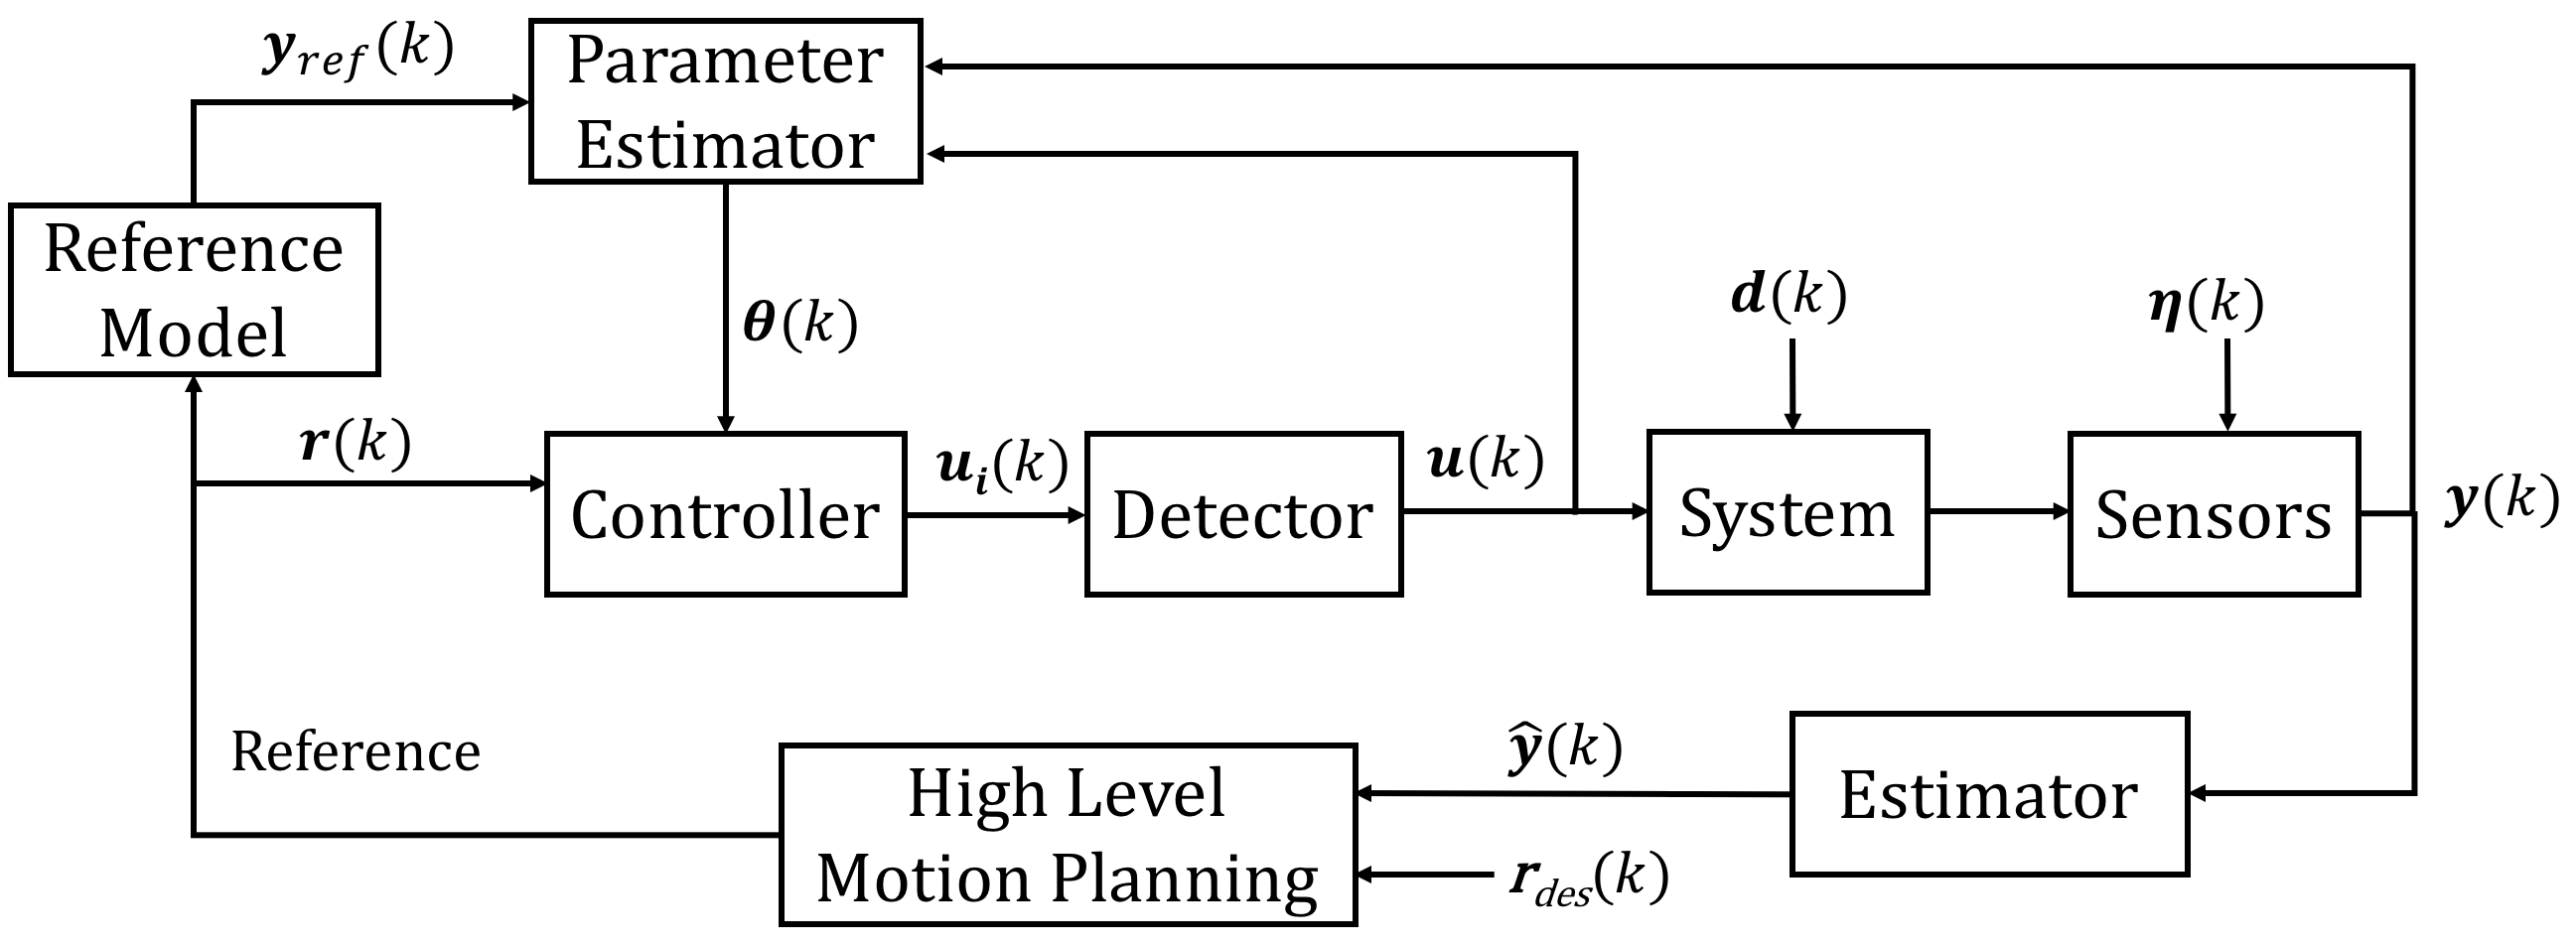
\includegraphics[width=0.46\textwidth]{sys_arch.png}
\caption{Overall system architecture showing the relationship between the reference model adaptive controller and the adaptive motion planner.}
\label{fig:system_arch}
\end{figure}

\subsection{Resilient Adaptive Control}
\label{sec:Res_adapt_control}

In this section \NB{avoid "In this section, In this work"} \NB{this first part can go in the previous section, something like: Next, we described the framework for attack detection and ...}we describe our framework to detect sensor attacks and the sensor reconfiguration problems using a series of adaptive controlled subsystems. 
\NB{In order to detect and remove attacks we propose the architecture in Fig. 2 in which redundant sensor measurements are considered. Specifically multiple subsystems are considered, one for each sensor measurement and whiting each subsystem a model reference adaptive control scheme is implemented to obtain the desired input to track a reference signal $y^*$. As in our previous work \cite{NICOLA IROS14 AND ICCPS14} here we assume that at most $N/2$ sensors can be compromised in order to estimate the state of the system.}
The architecture followed in this work is shown in Fig. \ref{fig:det_arch}, which consists of a subsystem for each sensor measurement within the same controlled state. Each subsystem consists of a model reference adaptive controller to generate the next input $u^*_i$ where $i=1,2,\dots,s$ given its corresponding measurement signal $y_i$.

First, to design the resilient model reference adaptive controller, we assume that:
	\begin{enumerate}[leftmargin=3\parindent]
	\item[$A1)$] all zeros of $B^{'}(z^{-1})z^q$ from \eqref{eq:B_prime} are within $|z|<1$. 
	\item[$A2)$] $p$ and $q$ are known. 
	\item[$A3)$] the system delay $d$ is known.
	\item[$A4)$] all poles of $E(z^{-1})z^w$ from \eqref{eq:reference model_z} are within $|z|<1$.
	\end{enumerate}
The zeros $z$ of the system are within the discrete $z-plane$ while $p$, $q$, and $d$ are the dimensions of \eqref{eq:transfer_function}. With these assumptions satisfied, every $i^{th}$ subsystem can generate an input signal $u^*_i(k)$ to have its measurement signal $y_i$ track a given tracking signal $y^*$ from the reference model \eqref{eq:reference model_z}. Many of the steps to design the Characteristic Model Based all-coefficient Model Reference Adaptive Controller are omitted here, which can be found in \cite{tao2003adaptive,Goodwin1643720}, however we provide the important\NB{main...avoid expressions like important, beautiful, awesome, incredible, etc} equations \NB{needed to compute next input $u(k+1)$}to calculate for the next input. A parameter vector of unknown coefficients describing the system's transfer function \eqref{eq:transfer_function} to follow the desired reference model is described as:
    \begin{equation}
	\bm{\theta}_0=(\alpha_0, \dots ,\alpha_{p-1},\beta_0, \dots ,\beta_{q+d-1})^T \in \R^{p+q+d}
	\end{equation}
The objective of the adaptive control is to estimate the true parameters of $\bm{\theta}_0$ with the parameter estimate vector $\bm{\theta}^T(k)$:
    \begin{equation}
    \bm{\theta}(k)=(\theta_1(k), \dots ,\theta_p(k),\theta_{p+1}(k), \dots ,\theta_{p+q+d}(k))^T
	\end{equation}
With our known input and measurement signals within a signal vector $\bm{\phi}(k)$,
    
	\begin{align}
	\begin{split}
	\bm{\phi}(k)&=(y_i(k), \dots ,y_i(k-p+1),u^*_i(k), \dots , \\
	& u^*_i(k-q-d+1))^T \in \R^{p+q+d}
	\end{split}
	\end{align}
we can estimate the true parameter vector $\bm{\theta}_0$ by updating the parameter estimate vector $\bm{\theta}^T(k)$ using a \textit{Modified Projection Algorithm}:
	\begin{equation}
	\label{eq:Modified_Proj_Algorithm}
	\bm{\theta}(k)=\bm{\theta}(k-1)+\frac{a(k)\bm{\phi}(k-d)e(k)}{c+\bm{\phi}^T(k-d)\bm{\phi}(k-d)}
	\end{equation}
	\begin{equation}
	e(k)=E(z^{-1})y_i(k)-\theta^T(k-1)\bm{\phi}(k-d)
	\end{equation}
	\begin{align*}
	\epsilon<a(k)<2-\epsilon, 0,\epsilon<1, c>0
	\end{align*}
To follow the desired tracking output $y^*(k)$ from the reference model, the adaptive control input $u^*_i(k)$ is then calculated from the equation:
    \begin{equation}
    \label{eq:tracking_model}
	\bm{\theta}^T(k)\bm{\phi}(k)=E(z^{-1})y^*(k+d)
	\end{equation}
By rearranging \eqref{eq:tracking_model} we isolate $u^*_i(k)$ to calculate our next input signal for each subsystem \NB{$i=1...complete$}:
	\begin{align}
	\label{eq:End}
	u^*_i(k)=\frac{1}{\theta_{p+1}(k)}&(-\theta_1(k)y_i(k)-\theta_2(k)y_i(k-1)  \nonumber \\
    -\dots-\theta_p(k)y_i(k&-p-1)-\theta_{p+2}(k)u^*_i(k-1)  \\
	-\theta_{p+3}(k)u^*_i(k-2)-& \dots - \theta_{p+q+d}(k)u^*_i(k-q-d+1) \nonumber \\
	+g&H(z^{-1})r(k))^T \nonumber
	\end{align}
    \begin{equation}
	\theta_{p+1}(k)\neq0 \nonumber
	\end{equation}

\NB{Once these subsystems inputs are computed, under the assumptions in (A1-A4), we leverage the following MRAC properties to detect...:}
We leverage many of the MRAC's assurances and guarantees for our technique to detect sensor attacks when the system model is changing or unknown. We know that under the assumptions of (A1-A4), the following are true \cite{tao2003adaptive},
	\begin{enumerate}[label=(\roman*),leftmargin=3\parindent]
	\label{assumtions_ensure}
	\item[$T1)$] $y(k)$ and $u(k)$ are bounded 
	\item[$T2)$] $\lim_{k\to\infty}(y(k)-y^*(k))=0$
	\label{Truth2}
	\item[$T3)$] $\sum_{k=0}^\infty(y(k)-y^*(k))^2<\infty$
	\end{enumerate}
where $y(k)$ is the system output and $y^*(k)$ is a tracking signal from the reference model. This ensures the system's output asymptotically converges to the reference model's tracking signal in a finite amount of time. 


The resilient adaptive controller employs the architecture of redundant subsystems where each sensor measurement $y_i$ has its adaptive controller to generate an input $u^*_i$ to follow a desired tracking signal $y^*_i$. Each of the sensor measurements, when uncompromised, have convergence (T2) towards their desired tracking signal from the corresponding reference model,
    \begin{equation}
    \label{multiple_output_tracking}
    \lim_{k\to\infty}(y_i(k)-y^*_i(k))=0
    \end{equation}
for $i=1,2,\dots,s$. This remains true with a changing reference signal $r_i(k)$, changing dynamics, or bounded disturbances. 

\begin{figure}[ht!]
\vspace{1pt}
\centering
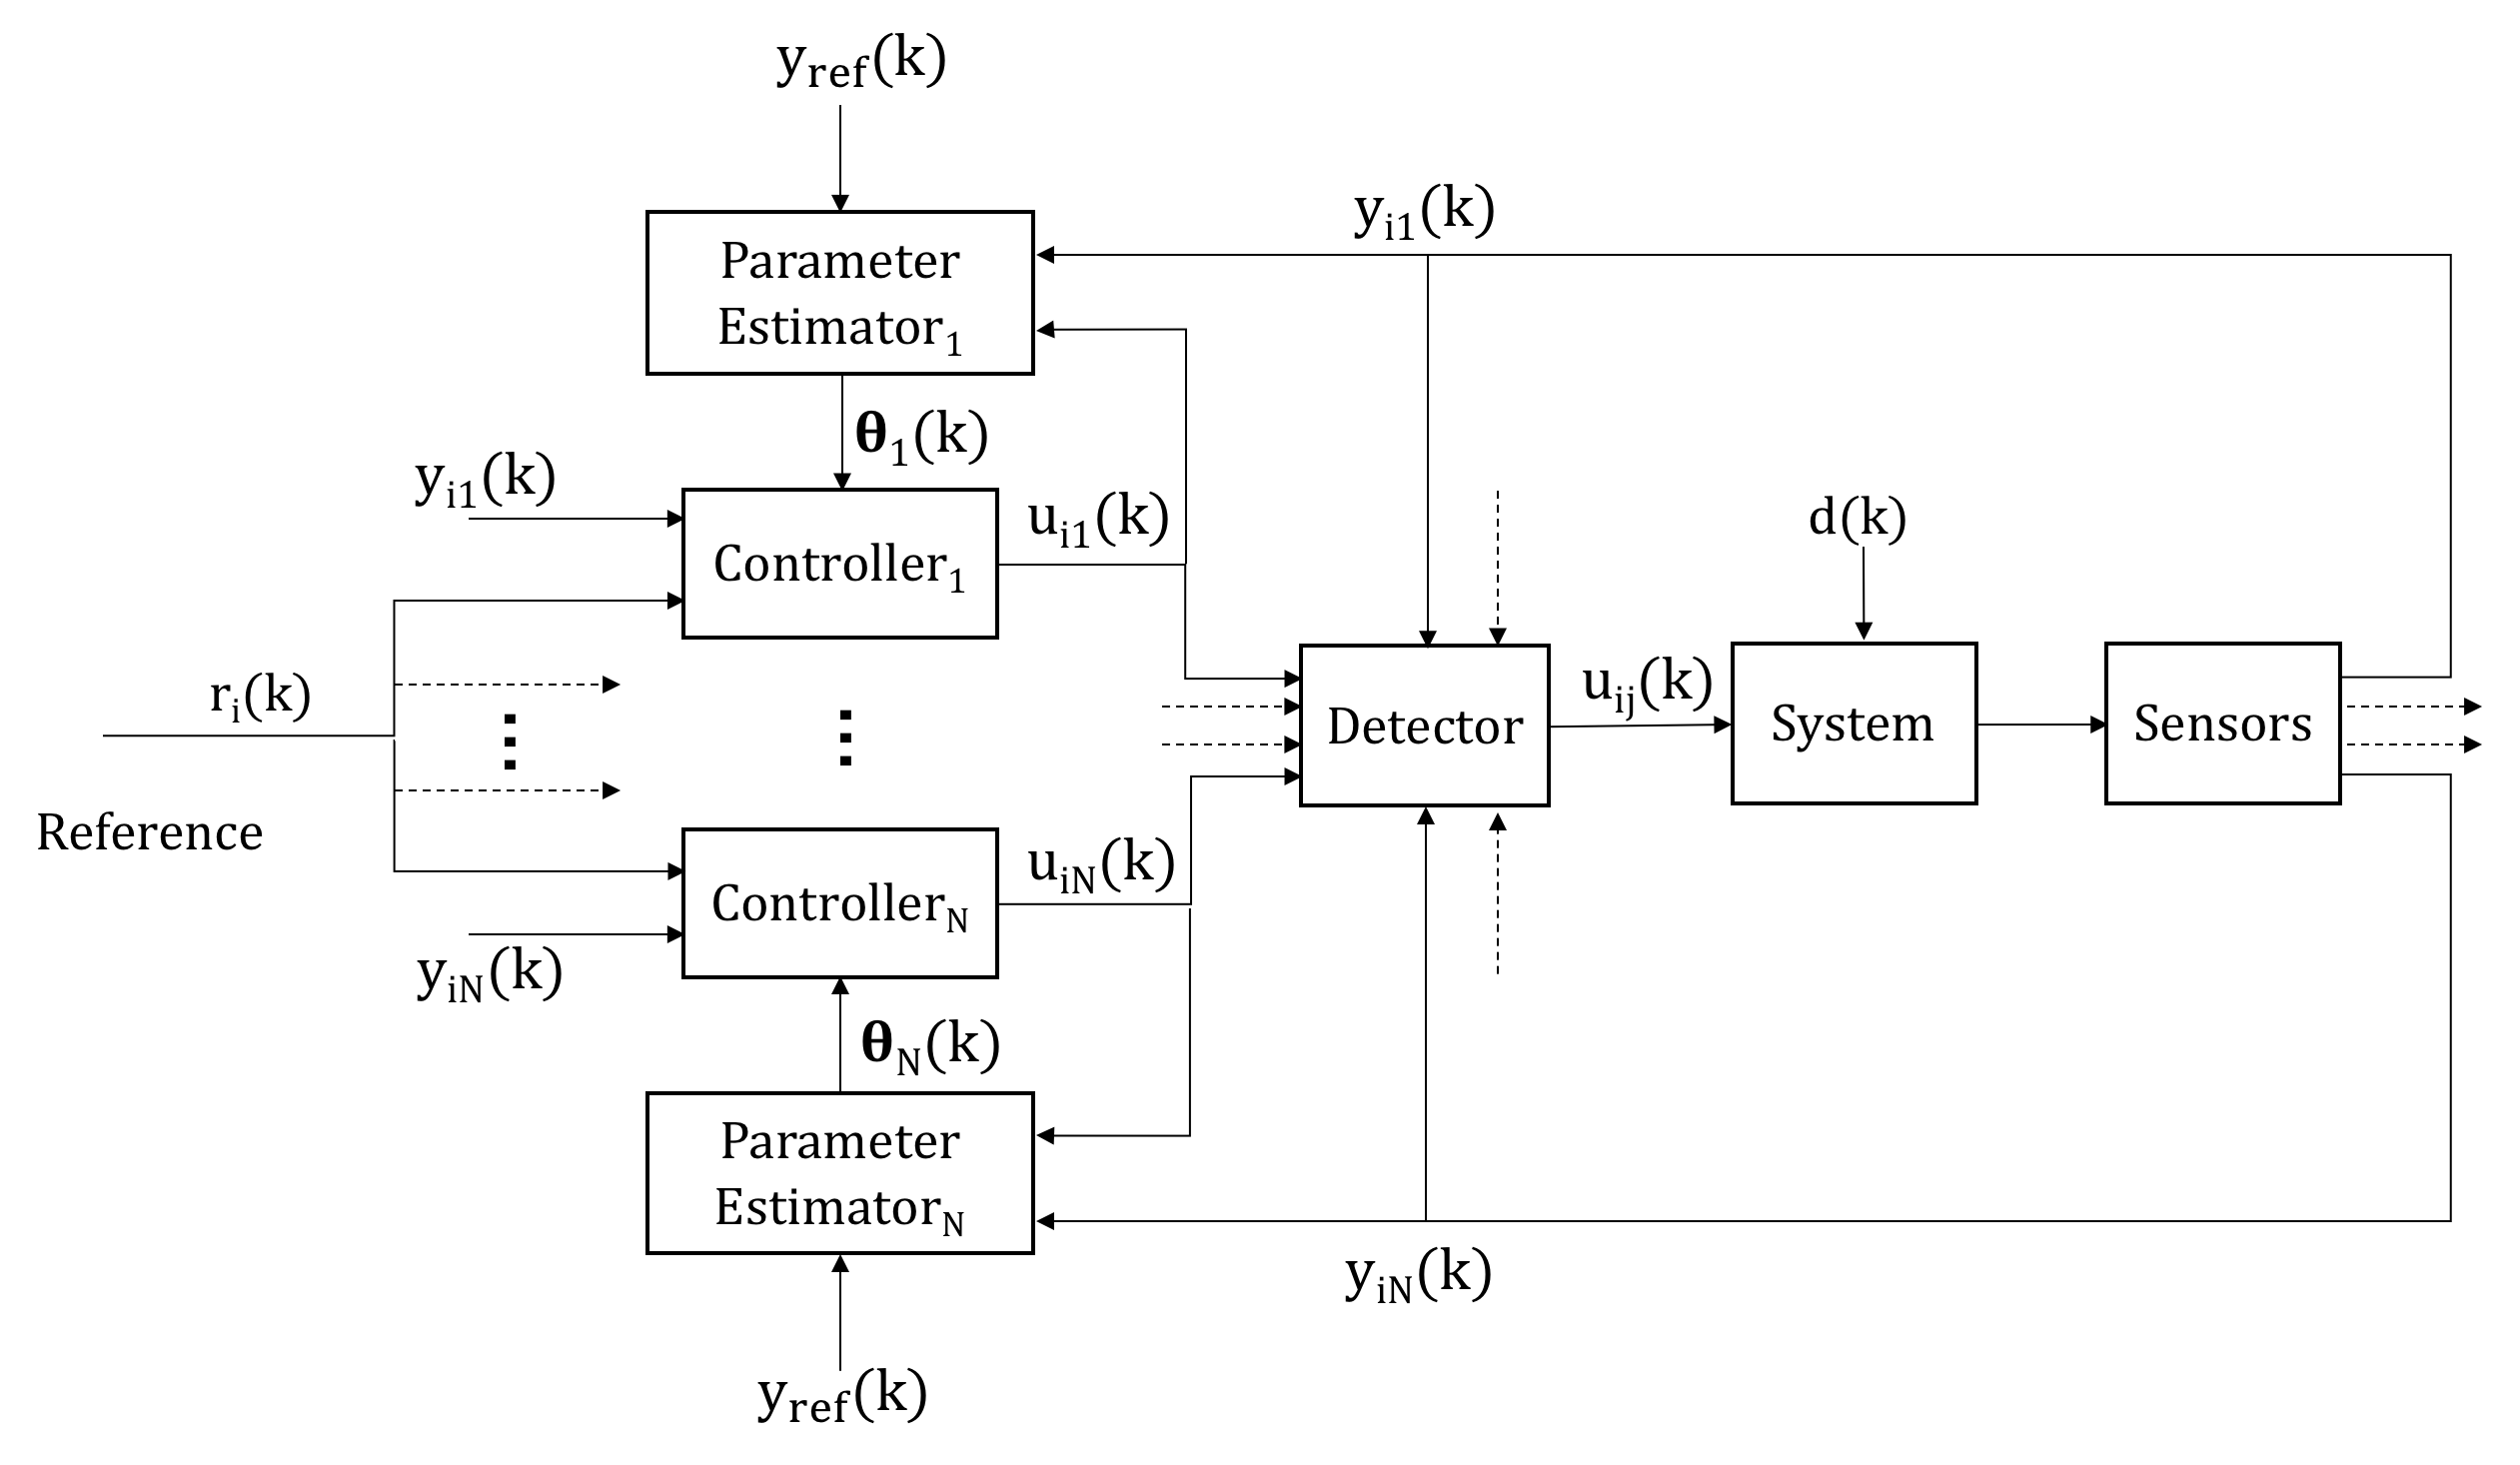
\includegraphics[width=0.48\textwidth]{con_and_det.png}
\caption{Architecture of the detection scheme within the adaptive controlled system. Representing  the $s$ number of available measurements, each of their adaptive subsystems generate a temporary input to be sent to the attack detector. From there, the detector removes measurement subsystems that are compromised.}
\label{fig:det_arch}
\end{figure}

%\eqref{eq:Start}$-$\eqref{eq:End}

	
As shown in Fig. \ref{fig:det_arch}, each $i^{th}$ MRAC subsystem has its own measurement signal, but they all share the same reference model and input $u(k)$ that is directly used to control the specific state. Each MRAC subsystem calculates an updated temporary input $u^*_i(k)$ that is fed into the detector, which analyses each to check for attacks. \NB{this section from "The resilient adaptive controller employs...till here" is confusing and redundant. Shrink it to the bare minimum and just add any new information or anything that may help to clarify if needed}

Since \eqref{multiple_output_tracking} should hold during any operation, the following is also true:
\begin{equation}
    \label{eq:u_to_0}
    \lim_{k\to\infty}(u^*_i(k)-u^*_j(k))=0, \text{ }i\neq j
\end{equation}
\NB{specify in the equation $i,j=1...N$}
where $u^*_i$ and $u^*_j$ refer to temporary inputs calculated from their respected subsystems\NB{to track the same signal $y_i^*(k)$. remove the rest} to control their measurement signal $y_i(k)$ towards the same tracking signal $y_i^*(k)$. Each temporary input, under ideal conditions, should be the same value as all other temporary inputs controlling their output to track the same tracking signal. For each subsystem to properly calculate the next input $u^*_i(k)$, their sensor measurement $y_i$ needs to be uncompromised. When one or more measurements have a non-zero value from the sensor attack vector $\xi_i(k) \neq 0$, those corresponding $i^{th}$ subsystem inputs $u^*_i$ diverge from the uncompromised subsystems.\NB{this last sentence is hard to read...fix it}

For attack detection, a difference matrix $\bm{\Psi}(k)$ is designed for every time interval $k$ of each controlled state. The structure of this matrix is,
    \begin{equation}
    \label{eq:error_matrix}
	\bm{\Psi}(k)=\begin{bmatrix} \psi_{1,1}(k) & \psi_{1,2}(k) & \dots & \psi_{1,s}(k) \\ \psi_{2,1}(k) & \psi_{2,2}(k) &  &  \\ \vdots &  & \ddots &  \\ \psi_{s,1}(k) &  &  & \psi_{s,s}(k) \end{bmatrix}
	\end{equation}
where $\bm{\Psi}(k) \in \R^{s\times s}$ with $s$ is \NB{"with s is" is not english}the number of measurements from the available measurement set $\bm{y} \in \R^s$. Each \NB{$\psi_{i,j}\in\bm{\Psi}$} element within $\bm{\Psi}(k)$ is \NB{computed as the absolute error between the two subsystem i and j inputs}represented as the absolute difference between two temporary inputs:
    \begin{equation}
        \psi_{i,j}(k)=|u^*_i(k)-u^*_j(k)|
    \end{equation}
\NB{use passive form as much as possible. The $l_1$ norm for each raw in ... is then computed which...}We take an $l_1$ vector norm of the $i^{th}$ row from the difference matrix \eqref{eq:error_matrix} which gives us the following difference vector:
    \begin{equation}
    \label{eq:difference_vector}
	\bm{\Psi^{'}}(k)=\begin{bmatrix} \lVert{\bm{\Psi}_1(k)}\rVert_1 \\ \lVert{\bm{\Psi}_2(k)}\rVert_1 \\ \vdots \\ \lVert{\bm{\Psi}_s(k)}\rVert_1 \end{bmatrix}
	\end{equation}
Let's consider the minimum valued element of \eqref{eq:difference_vector} to form another vector $\bm{\Psi}^{'}_{min}(k) \in \R^s$, with every element equal to $\min \bm{\Psi}^{'}(k)$:
    \begin{equation}
	\bm{\Psi}^{'}_{min}(k)=\begin{bmatrix} \min \bm{\Psi}^{'}(k),& \dots \text{ },&\min \bm{\Psi}^{'}(k) \end{bmatrix}^T
	\end{equation}
We now define the updated error vector as:
    \begin{align}
    \label{eq:Psi2}
	\bm{\Psi^{''}}(k)&=\bm{\Psi^{'}}(k)-\bm{\Psi}^{'}_{min}(k) \\
	& =\begin{bmatrix} \lVert{\bm{\Psi}_1(k)}\rVert_1 - \min \bm{\Psi}^{'}(k)\\ \lVert{\bm{\Psi}_2(k)}\rVert_1 - \min \bm{\Psi}^{'}(k) \\ \vdots \\ \lVert{\bm{\Psi}_s(k)}\rVert_1 - \min \bm{\Psi}^{'}(k) \end{bmatrix}
	\end{align}
	
From \eqref{eq:u_to_0} while under ideal conditions (i.e., with no noise), the error vector \eqref{eq:Psi2} has all elements equal to zero. When an $i^{th}$ sensor is under attack, the $i^{th}$ input diverges from the remaining uncompromised inputs. The $i^{th}$ element of $\bm{\Psi}^{''}(k)$ becomes non-zero due to the compromised sensor, while the rest of the elements remain zero. 

Under non-ideal conditions where noises exist, the elements of the error vector will not remain zero while sensors are uncompromised. By setting a threshold value $\delta$, we say \NB{NO NO NO NO...in papers we don't say anything�} all elements of the error vector need to stay below this level. By refining \eqref{eq:Psi2} for non-ideal conditions we get,
    \begin{align}
    \begin{split}
    \label{eq:Psi2_nonideal}
	\bm{\Psi^{''}}(k)&=\bm{\Psi^{'}}(k)-\bm{\Psi}^{'}_{min}(k) \\
	& =\begin{bmatrix} \lVert{\bm{\Psi}_1(k)}\rVert_1 - \min \bm{\Psi}^{'}(k)\\ \lVert{\bm{\Psi}_2(k)}\rVert_1 - \min \bm{\Psi}^{'}(k) \\ \vdots \\ \lVert{\bm{\Psi}_s(k)}\rVert_1 - \min \bm{\Psi}^{'}(k) \end{bmatrix} \leq \bm{\delta}
	\end{split}
	\end{align}
with the vector $\bm{\delta} \in \R^s$ has elements all equal to the scalar value $\delta$\NB{how is $\delta$ computed...show}. When an $i^{th}$ element of $\bm{\Psi^{''}}(k)$ breaks the $\delta$ threshold, the corresponding $i^{th}$ measurement is placed into the set $\bm{y}_a$ for measurements no longer used by the system. The updated measurement set is $\bm{y}=\bm{y}_0\setminus\bm{y}_a$ where $\bm{y}_0$ was the initial full set of measurements and $\bm{y}_a$ is the set of removed measurements due to attacks. The updated measurement vector is of the dimensions $\bm{y} \in \R^{s}$ with $\bm{s}_0$ as the initial set of sensor measurements and $s_a$ representing the size of attacked sensor measurement set $\bm{y}_a$ \NB{this sentence is odd...remove it}. The new dimension of the output matrix due to the changing measurement vector is $\bm{C} \in \R^{s\times n}$ where $s=s_0-s_a$ \NB{all of the above overcomplicated sentences can be summarized as: After detecting and removing the compromised sensors, the updated measurement matrix shrinks to $\bm{C} \in \R^{s'\times n}$ with $s'=s_0-s_a$}. Effective detection is constrained to when less than half of the measurements of the same controlled state are attacked \NB{we state this before, also "to when" not good grammar}. Once all temporary \NB{why temporary? Are there not temporary inputs in this work? What's a temporary input?} inputs $u_i^*(k)$ have been checked, the best available (e.g. measurement with lowest noise profile) is chosen to be used for the true control signal $u_i(k)$ to the system.\NB{red flag here.How is this obtained?}



% DO I NEED THIS?

%Properties of the modified projection algorithm \eqref{eq:Modified_Proj_Algorithm} include:
%    \begin{enumerate}[label=(\roman*),leftmargin=3\parindent]
%	\item every iteration improves estimation:
%	    \begin{align}
%	        \|\bm{\theta}(k)-\bm{\theta}_0\|\leq\|\bm{\theta}(k-1)-\bm{\theta}_0\|, k\geq1 \nonumber
%	    \end{align}
%	\item parameter variation converges to zero:
%	    \begin{align}
%	        \lim_{k\to\infty}(\bm{\theta}(k)-\bm{\theta}(k-N))=0, \text{any finite } N>0 \nonumber
%	    \end{align}
%	\end{enumerate}
	
%(TALK ABOUT PERSISTENT EXCITATION BRIEFLY)
	

\subsection{Estimation Confidence}

In this work \NB{remove in this work. It kills the fluidity of the paper} we leverage the statistical technique of confidence intervals \cite{devore2011probability} to obtain a specific confidence of an estimate \NB{why? what's the problem here? Why do we need this? Please be clear and present the issues, something like...The vehicle has multiple sensors with different noise profiles, some of which are fused to obtain better state estimation, for example using Kalman filtering techniques. If a sensor is compromised, our detection scheme will remove it, however leaving the system with a smaller set of sensors. Thus here we are interested to compute a confidence interval around our state estimation and adapt the vehicle's motion plan if safety constraints could be violated.}. Confidence intervals are important because they calculate a confidence percentage that the true mean lies within the estimated bounds. As the number of data samples increases, the confidence interval shrinks in size to give a better estimation of the true mean \NB{you are giving the results before showing how!}. Assuming the knowledge of the confidence percentage $z^{*}$ \NB{change symbol, confusing with previous z}, population standard deviation $\sigma$, the number of sensor data samples $N$, and the mean of the $N$ sensor data samples $\bar{x}$, an interval of a percentage of confidence can be calculated:
    \begin{equation}
     \label{Confidence_interval}
		C_x = \bar{x} + z^{*}\frac{\sigma}{\sqrt{N}}
	\end{equation}
	
For position estimation with sensor uncertainties, we need a guarantee the vehicle is within a region to prevent navigation into an undesired state. To do this, \NB{avoid as much as possible these opening "to do this"} uncompromised sensor measurements are fused using filtering techniques (e.g. Kalman Filtering) and the result is a position estimate $\hat{\bm{p}}=[\hat{x},\hat{y}]^T$ of a certain variance $\sigma_p^2$, which depends on the known sensor variances from data sheet specifications. Using an $N$ number of data samples of variance $\sigma_p^2$, we are able to estimate an interval of specific confidence that the vehicle is within the these boundaries \NB{rewrite better please, not clear}.

For our case, we want to estimate a 2-dimensional interval. By calculating this multivariate confidence interval, we name it a confidence region, we estimate a region which the vehicle is within \NB{rewrite, terrible form.} \NB{I'm stopping here. This last part is really bad written. Rewrite in good english and form!}. This method guarantees the center of the vehicle has a specific percentage of confidence that it's within this region. The data being used for estimation has the form $\mathcal{N}(0,\sigma_p)$ where the position estimate data's population standard deviation $\sigma_p$ is known for any sensor combination. Using \eqref{Confidence_interval} we can find a multivariate region of a determined confidence percentage that the vehicle is within to ensure safety,
    \begin{equation}
    \label{Confidence_region}
		\hat{\bm{\varepsilon}}_{\hat{\bar{\bm{p}}}|N} = \hat{\bar{\bm{p}}} + c_p\frac{\sigma_p}{\sqrt{N}}
	\end{equation}
with $c_p$ defining the value for a specific confidence percentage, which can be found in $z$-tables and $t$-tables in \cite{devore2011probability}. The radius of the multivariate confidence region \eqref{Confidence_region} is:
    \begin{equation}
		\hat{\varepsilon} = c_p\frac{\sigma_p}{\sqrt{N}}
	\end{equation}
Similar to the calculation of confidence intervals, it is under the assumption the true mean is static, is not changing over time. This cannot be assumed in our case of position estimation of a navigating vehicle. 

% \begin{figure}[ht!]
% \vspace{1pt}
% \centering
% 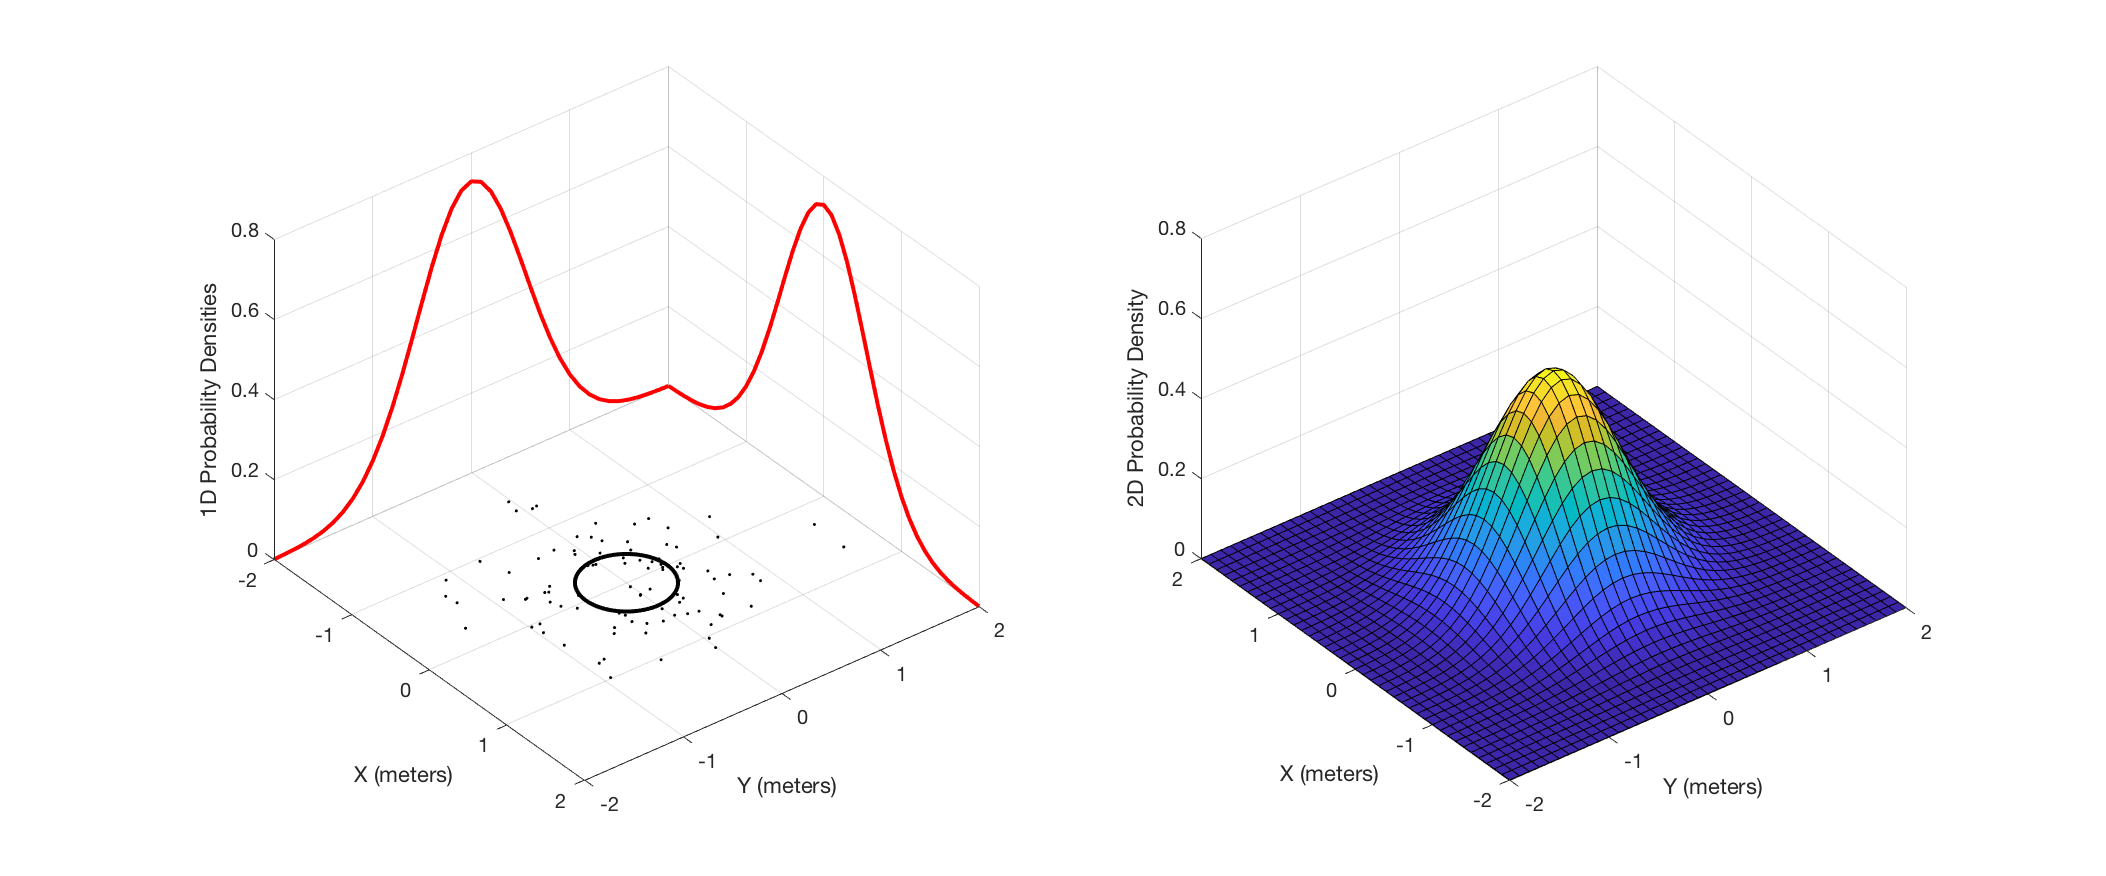
\includegraphics[width=0.48\textwidth]{Gaussian2D.png}
% \caption{Distribution of vehicle's estimated position over 100 samples in an $X-Y$ plane with equal noise variance on the $X$ and $Y$ axis. Creating a psuedo-static case allows for the calculation of a confidence region for vehicle position.}
% \label{fig:gauss_pdf}
% \end{figure}


\begin{figure}[ht!]
\label{fig:gauss_pdf}
\begin{tabular}{cc}

\subfigure[\label{fig:1sample} ]{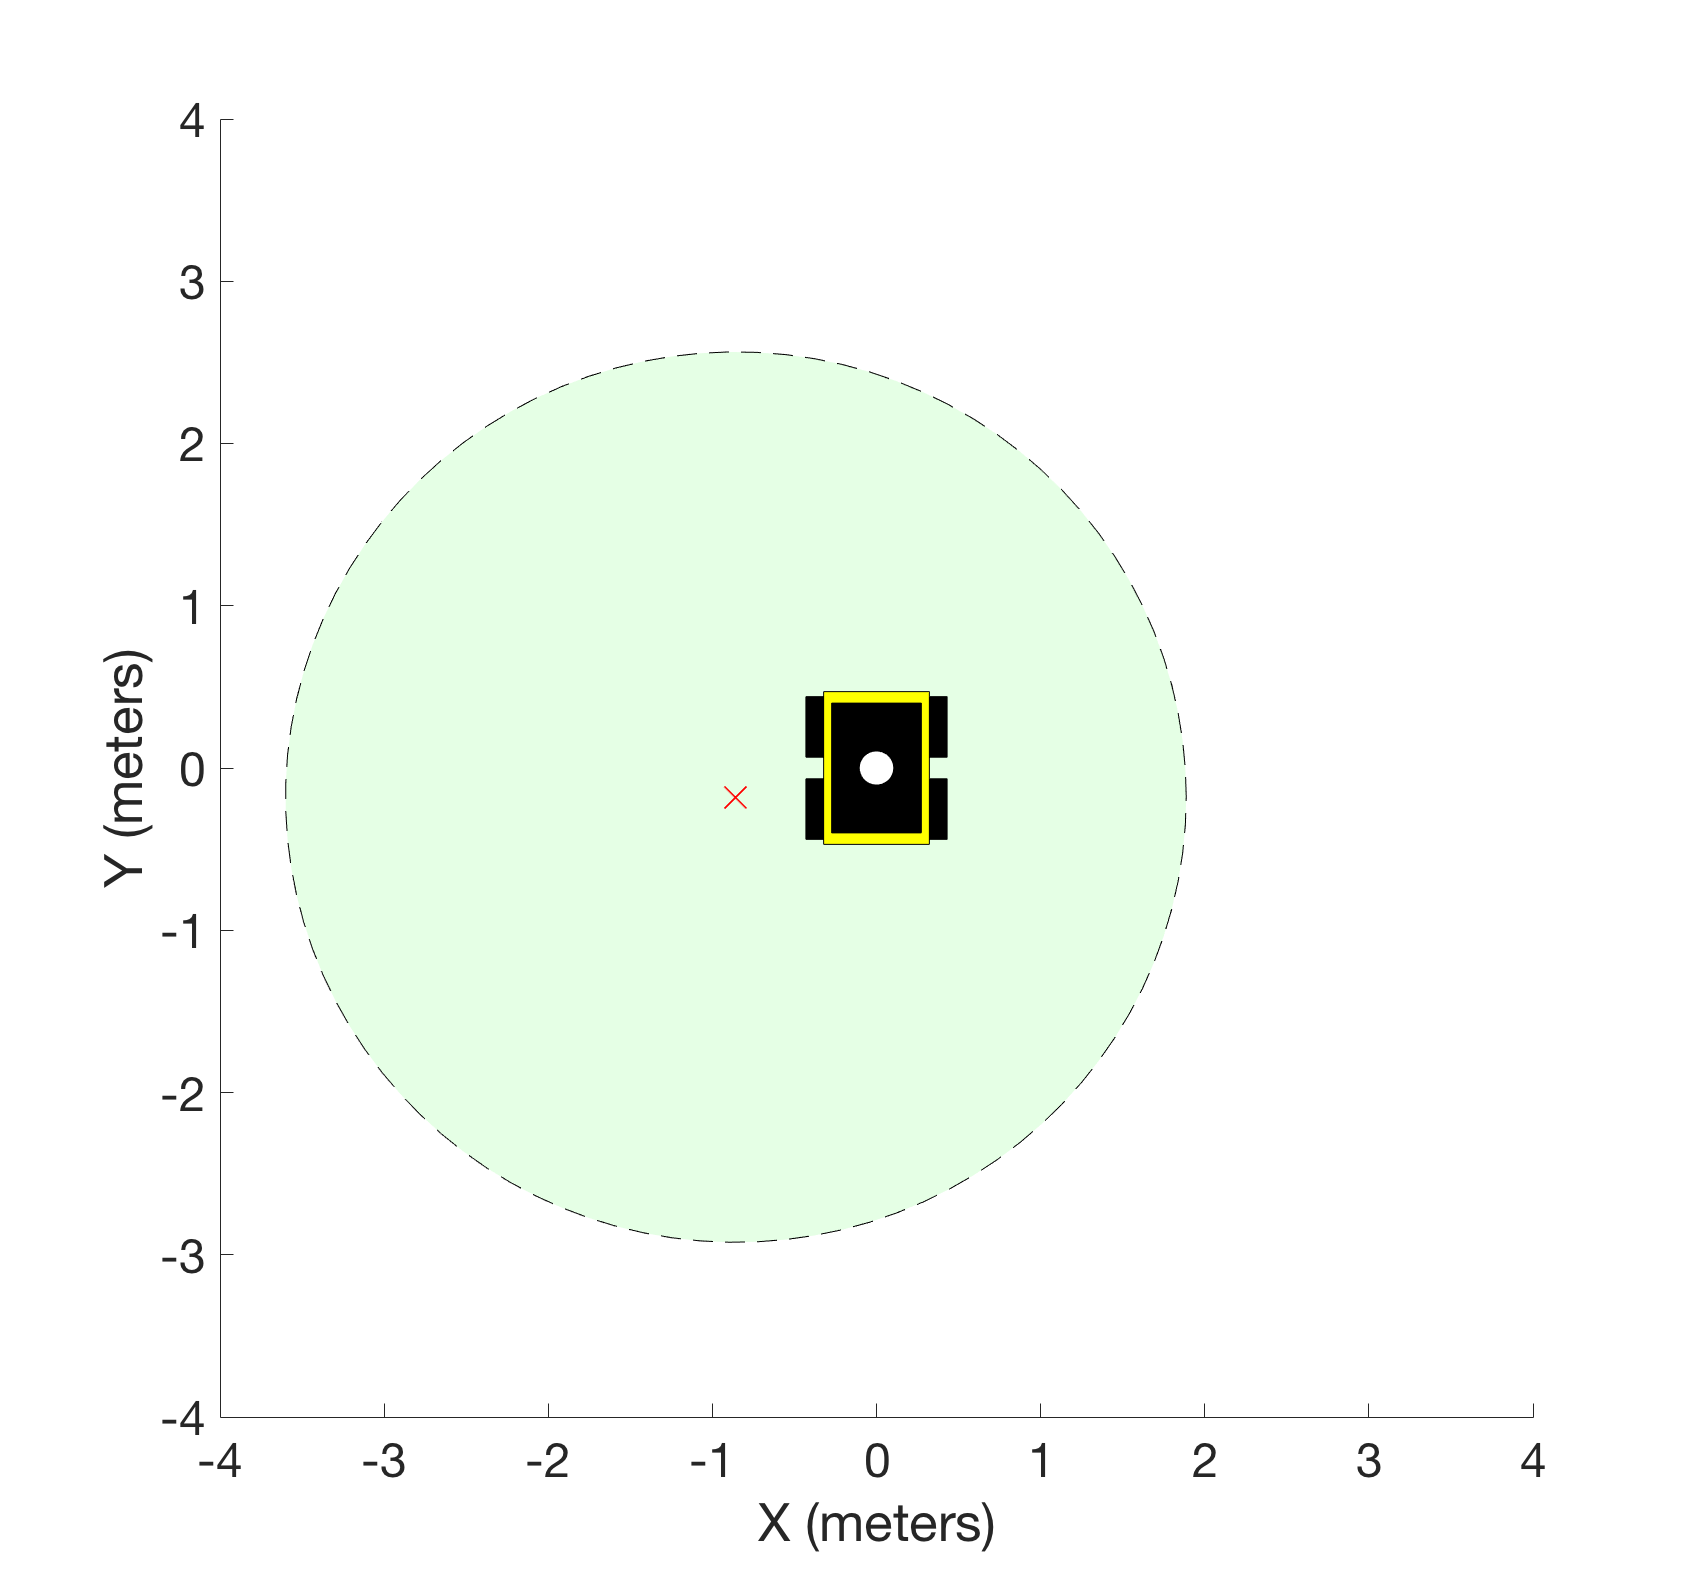
\includegraphics[width = 0.22\textwidth]{sample1.png}} &	

\subfigure[\label{fig:5samples} ]{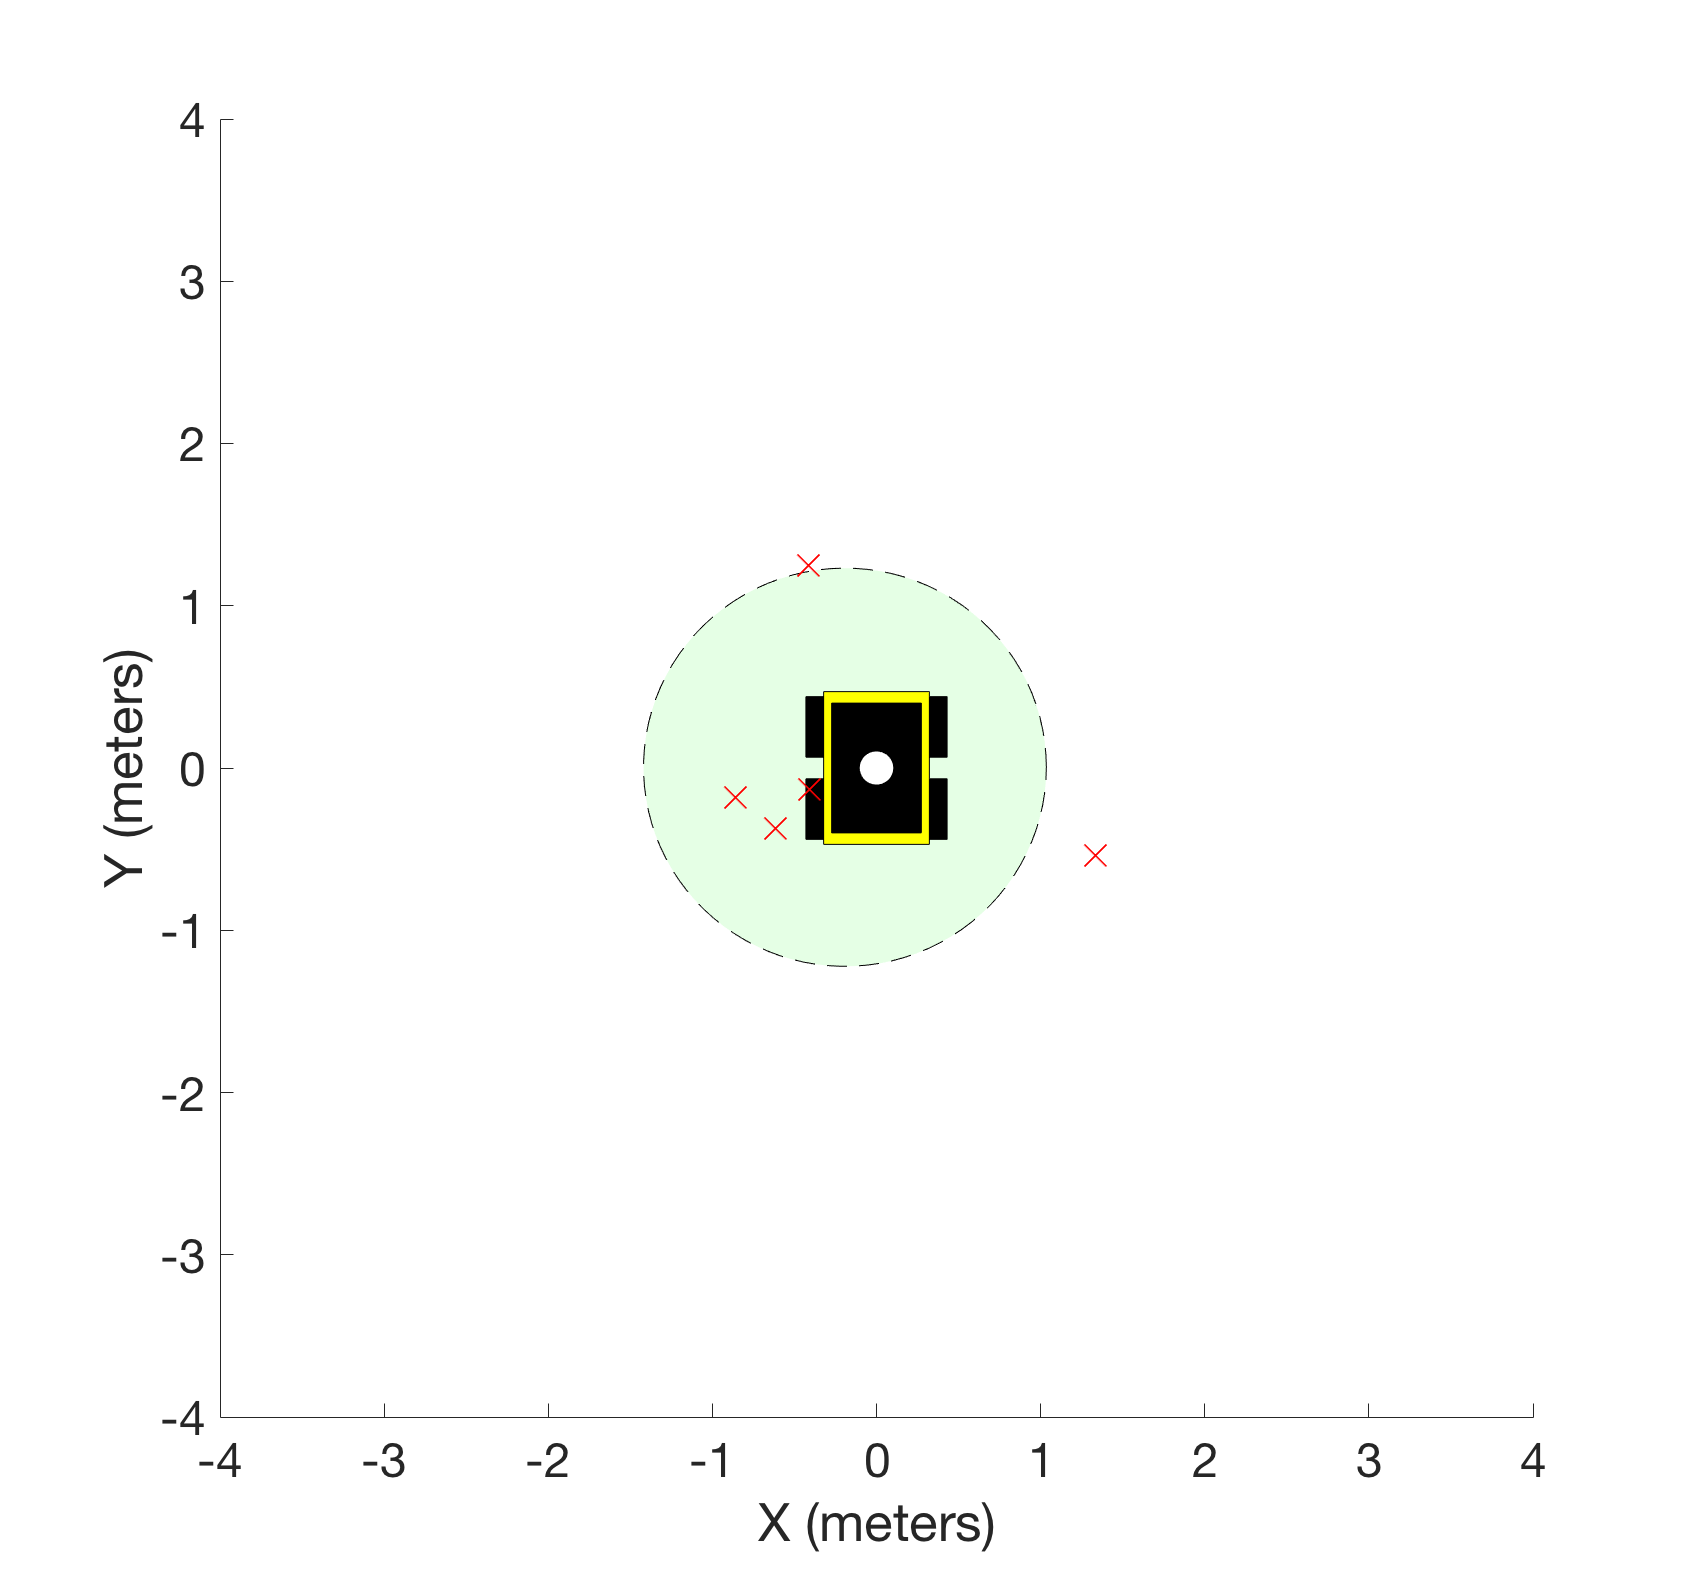
\includegraphics[width = 0.22\textwidth]{sample5.png}}

\end{tabular}
\caption{A comparison of the size of the estimated confidence region as the $N$ number of data samples grow. In \ref{fig:1sample}, the estimated confidence region with 1 data sample is not as accurate. In \ref{fig:5samples}, the $N$ number of samples used is five, which gives a much smaller size and more accurate confidence region.}

\end{figure}

A pseudo-static form of a confidence region is made to compensate for translation of previous position measurements $\hat{\bm{p}}(k-i)$, where $i=1,2,\dots,N-1$. These $N-1$ number of previous position data points need to be represented as if they were all sampled for the current position in time $k$, creating a pseudo-static set of data to calculate the confidence region. As shown in Fig. \ref{fig:gauss_pdf}, we want to have the data samples for calculation of the confidence region look as if the vehicle is stationary. The $N$ position estimate samples are described in the set,
\begin{equation}
    \hat{\bm{P}}=\begin{bmatrix} \hat{\bm{p}}(k) ,\hat{\bm{p}}(k-1),\dots,\hat{\bm{p}}(k-N+1) \end{bmatrix} 
\end{equation}
for the position coordinates in the $x$ and $y$ direction. Translating the data coordinates into a pseudo-static form will create the updated set,
\begin{equation}
    \hat{\bm{P}}^*=\begin{bmatrix} \hat{\bm{p}}^*(k) ,\hat{\bm{p}}^*(k-1),\dots,\hat{\bm{p}}^*(k-N+1) \end{bmatrix} \nonumber
\end{equation}
Each element of these updated sets are calculated as,
	\begin{equation}
	\hat{\bm{p}}^*(k-i) = \hat{\bm{p}}(k-i)+\sum_{j=i}^1 v(k-j)\theta_h(k-j)t_s 
	\end{equation}
where $i=1,2,\dots,N-1$ and the most recent position estimate at time instant $k$ is unchanged from $\hat{\bm{p}}(k)$ to $\hat{\bm{p}}^*(k)$. The mean of the updated set is written as $\hat{\bar{\bm{p}}}^*$, which is used for the calculation of the estimated confidence region. To demonstrate how this works, Fig. \ref{fig:pseudo_static} gives a visualization of how the position estimates are transitioned into a pseudo-static case. Updating \eqref{Confidence_region}, we get
    \begin{equation}
    \label{Confidence_region_updated}
		\hat{\bm{\varepsilon}}_{\hat{\bar{\bm{p}}}^*|N} = \hat{\bar{\bm{p}}}^* + C_p\frac{\sigma_p}{\sqrt{N}}
	\end{equation}
 to account for all $N-1$ translated previous data points to appear as if they all were sampled at time interval $k$.

% \begin{figure}[ht!]
% \vspace{1pt}
% \centering
% 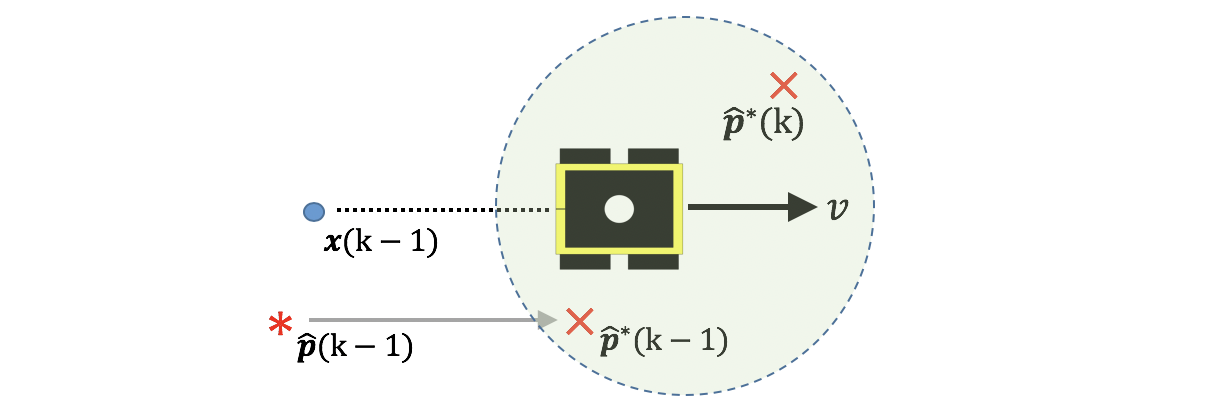
\includegraphics[width=0.48\textwidth]{pseudo_static.png}
% \caption{Translation of the original position estimates $\hat{\bm{p}}$ to a pseudo-static case $\hat{\bm{p}}^*$ as if all the position estimates were sampled from the vehicle at the current time interval $k$.}
% \label{fig:pseudo_static}
% \end{figure}


\begin{figure}[ht!]
\label{fig:pseudo_static}
\begin{tabular}{cc}

\subfigure[\label{fig:step_one} ]{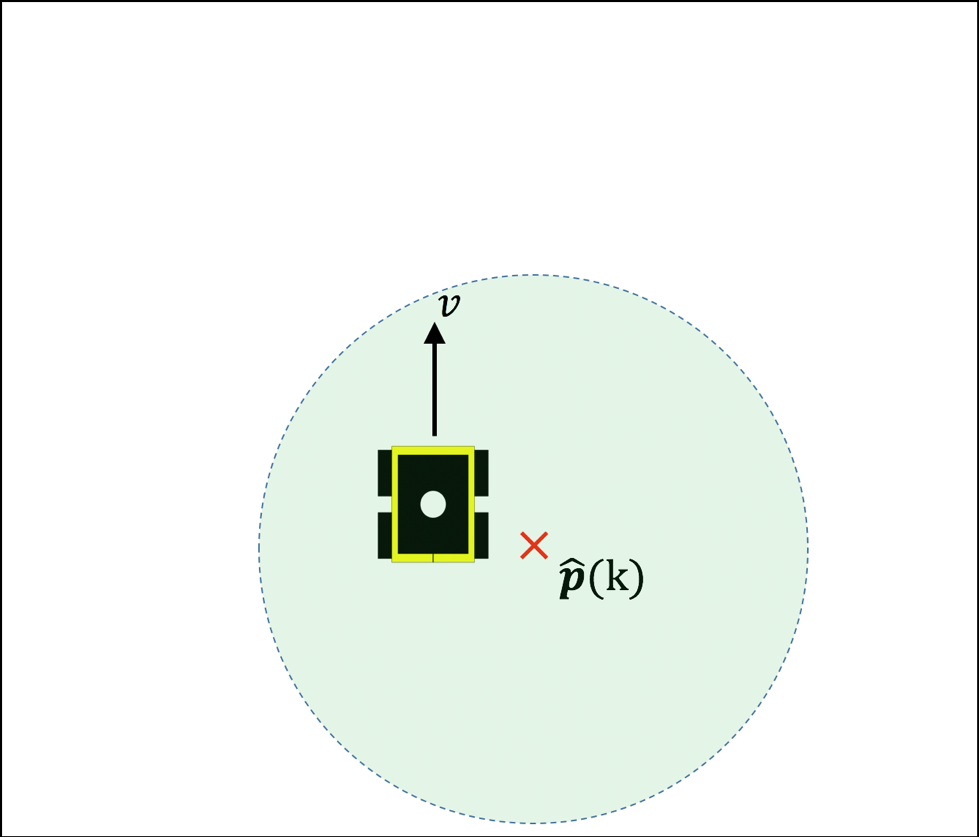
\includegraphics[width = 0.21\textwidth]{pseudo_static_left.png}} &	

\subfigure[\label{fig:step_two} ]{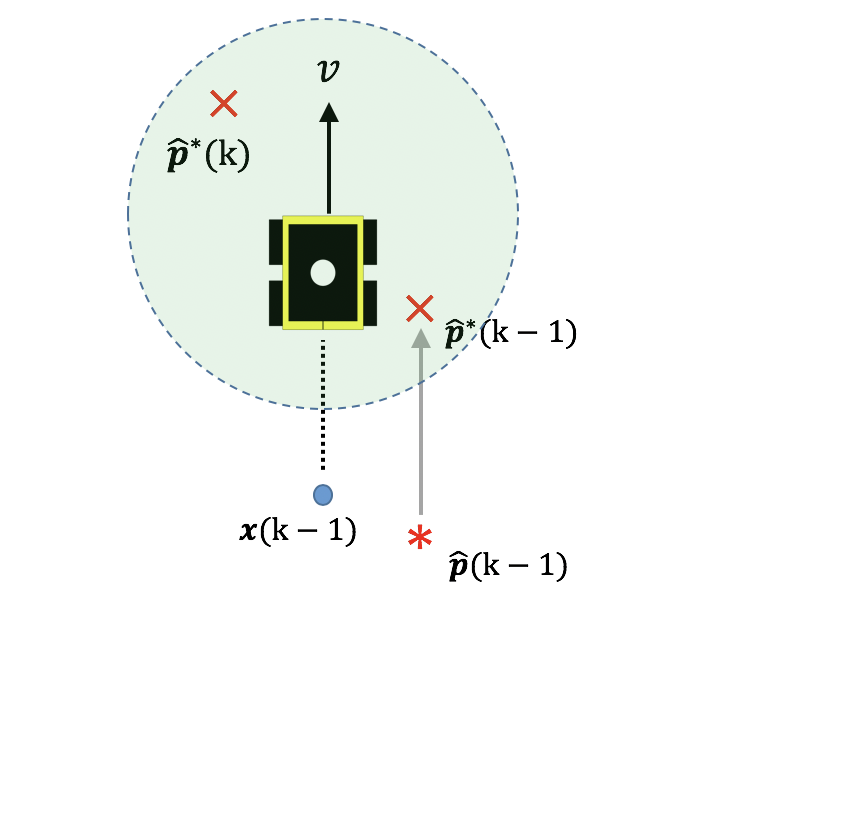
\includegraphics[width = 0.21\textwidth]{pseudo_static_right.png}}

\end{tabular}
\caption{Translation of the original position estimates $\hat{\bm{p}}$ to a pseudo-static case $\hat{\bm{p}}^*$ as if all the position estimates were sampled from the vehicle at the current time interval $k$.}

\end{figure}



Creating a pseudo-static case with these past position data samples introduces higher uncertainty. Uncertainties regarding the velocity sensor $\sigma_v$ and heading angle sensor $\sigma_h$ need to be accounted for. To guarantee the true position of the vehicle is within the estimation radial bounds, the maximum error in position due to the actuator and sensor noises over the furthest sample in time in $\hat{\bm{P}}^*$ is calculated as:
    \begin{align}
    \begin{split}
	\hat{\varepsilon}_{v,\theta_h|N}^{*}=\Big( \big[(\bar{v}^*& \cos{\bar{\theta}_h^*} - \bar{v}\cos{\bar{\theta}_h})(N-1)t_s \big]^2 \\
	&+ \big[ (\bar{v}^* \sin{\bar{\theta}_h^*} - \bar{v}\sin{\bar{\theta}_h})(N-1)t_s \big]^2 \Big) ^{1/2}
	\end{split}
	\end{align}
where,
    \begin{equation}
	\bar{v}^{*}=\bar{v}(k-i_{\varepsilon^{*}})+c_p\sigma_v \nonumber
	\end{equation}
    \begin{equation}
	\bar{v}=\bar{v}(k-i_{\varepsilon^{*}}) \nonumber
	\end{equation}
	\begin{equation}
	\bar{\theta}_h^{*}=\bar{\theta}_h(k-i_{\varepsilon^{*}})+c_p\sigma_h \nonumber
	\end{equation}
	\begin{equation}
	\bar{\theta}_h=\bar{\theta}_h(k-i_{\varepsilon^{*}}) \nonumber
	\end{equation}
with $i_{\varepsilon^{*}}=[1,2,,\dots,N-1]$ while average measured velocity and average measured heading angles over the past $N-1$ samples of range $i_{\varepsilon^{*}}$ are denoted by $\bar{v}$ and $\bar{\theta}_h$, respectively. Doing this account for velocity and heading angle measurement error and ensure the vehicle's position is within our estimation region.


\subsection{Adaptive Motion Planning}
With uncertainty of sensor measurements, with or without the loss of a compromised sensors, there needs to be guarantees to safely navigate a vehicle without accidents. As the vehicle approaches undesired regions or has a trajectory to follow through a passageway that's more narrow than the confidence region at the current time interval $k$, we need to be able to reduce the size of estimate region to guarantee safety. The only two options are to sample data faster or reduce speed to gather more samples within a certain distance. Since sampling at a faster rate can't be done, we need to slow the vehicle down to gather more data samples in a shorter distance to reduce estimation uncertainties.

To keep the vehicles estimated confidence region from intersecting with an unwanted region, a change to the number of current and past data samples in the calculation as well as an adaptation of the velocity. Without uncertainty of velocity and heading angle measurements, the equation to solve for the number of required $N$ samples to keep the confidence region within a specific radius is:
    \begin{equation}
    \label{conf_region1}
	    N^* = \left(c_p \frac{ \sigma_p }{ {\min \lVert \bm{x}_r - \hat{\bar{\bm{p}}}^* \rVert} -\Delta(k) } \right)^2
	\end{equation}
where $ \min \lVert {\bm{x}_r-\hat{\bar{\bm{p}}}^*} \rVert$ is the distance from the closest undesired region to the estimated vehicle center point position $\hat{\bar{\bm{p}}}^*$.
With the assumption of Normally distributed sensor noise on the velocity and heading angle sensors, the above equation is not suitable. The uncertainty region $\hat{\varepsilon}_{v,\theta_h|N}^{*}$ from these sensors must be accounted for. The revision to equation (\ref{conf_region1}) for a sufficient value of $N$ is:
    \begin{equation}
	    N^* = \left(c_p \frac{ \sigma_p }{ {\min \lVert \bm{x}_r - \hat{\bar{\bm{p}}}^* \rVert} -\hat{\varepsilon}_{v,\theta_h|N}^{*}-\Delta(k) } \right)^2
	\end{equation}
Due to the fact that $N^*$ represents the number of samples needed to reduce the estimation region to a desired size, $N^*$ needs to be an integer. We simply round $N^*$ up to the nearest integer to give us $N \in \N$.

An update of the reference velocity needs to occur when these undesired regions are within the entire confidence estimation region $ \hat{\varepsilon}_{\hat{\bar{\bm{p}}}^*|N} +\hat{\varepsilon}_{v,\theta_h|N}^{*}+\Delta(k)$ when $N=1$ to ensure the vehicle slows to capture more previous data samples with less estimation error. This reference velocity $r_v(k)$ update is calculated by:
    \begin{equation}
	    r_v(k)=r_v(k-1) \left[ \frac{ \min \lVert \bm{x}_r - \hat{\bar{\bm{p}}}^* \rVert - \hat{\varepsilon}_1}{\hat{\varepsilon}_2 - \hat{\varepsilon}_1} \right]
	\end{equation}
	\begin{equation}
	\begin{split}
	    \hat{\varepsilon}_1&=\hat{\bm{\varepsilon}}_{\hat{\bar{\bm{p}}}^*|N} +\hat{\varepsilon}_{v,\theta_h|N}^{*},\\ &\hat{\varepsilon}_2=\hat{\varepsilon}_1+\Delta(k) \nonumber	    
	\end{split}
	\end{equation}
	
where $\hat{\varepsilon}_1$ and $\hat{\varepsilon}_2$ are both radii from the estimated center position $\hat{\bar{\bm{p}}}^*$.
	
%	\begin{equation}
%		\Delta(k)=[v(k)]^{\delta_v}\delta
%	\end{equation}
%where $[\delta, \delta_v] \in R^{\geq0}$ are chosen values that determine the desired distance between the closest unwanted region to the estimation region as a function of velocity.


% INSERT ALGORITHM FOR REPLANNING VELOCITY
\begin{algorithm}
   \caption{Adaptive Motion for Safe Navigation} 
   \label{alg:adapt_motion} 
    \begin{algorithmic}[1]
	\State Initial conditions of system: $k=0$,$\bm{x}(0)=\bm{x}_0$
	\State Set $r_v(0)$ to desired velocity $r_{des}$
    \While{$1<k\leq\infty$}
        \State \Longunderstack[l]{ Calculate $\hat{\bar{\bm{p}}}^*$ then measure closest distance\\ to undesired region $\min \lVert \bm{x}_r - \hat{\bar{\bm{p}}}^* \rVert$.}
        \State Calculate radii of intervals $\hat{\varepsilon}_1$ and $\hat{\varepsilon}_2$ for $N$.
        \If{ $\min \lVert \bm{x}_r - \hat{\bar{\bm{p}}}^*\rVert < \hat{\varepsilon}_2(k)$}
            \State Solve for $N$ of next iteration
            \State Update reference for velocity $r_v(k)$
        \Else
            \If{$\min \lVert \bm{x}_r - \hat{\bar{\bm{p}}}^*\rVert < \hat{\varepsilon}_2(k)$ when $N=1$}
                \State Solve for $N$ of next iteration
                \State Update reference for velocity $r_v(k)$
            \Else
                \If{$r_v(k) \neq r_{des}$}
                    \State Reference velocity $r_v(k)=r_{des}$
                    \State $N = 1$
                \Else
                    \State Reference velocity $r_v(k) = r_v(k-1)$
                    \State $N = 1$
                \EndIf
            \EndIf
        \EndIf
    \EndWhile
	\end{algorithmic}
\end{algorithm}



\end{section} 